\chapter{Background}
\label{ch:theoreticalbackground}
The main concepts of this research are the \gls{ps}, \acrlong{ea}, and \gls{antifragile}. These three concepts are defined to create a common understanding. However, all three concepts use another concept. This concept is \textit{'system'}. For mutual understanding, the definition of system helps in understanding the \gls{ps}, \acrfull{ea}, and \gls{antifragile}.
\section{System}
\label{sec:tbsystem}
The main concepts of this research are the \gls{ps}, \acrlong{ea}, and \gls{antifragile}. These three concepts are defined to create a common understanding. However, all of these three concepts use another concept. This concept is \textit{'system'}. The definition of system helps in understanding the \gls{ps}, \acrfull{ea}, and \gls{antifragile}. Literature often uses the same concept but with a different meaning \parencite[p.~37]{Lapalme2012}. System is used for many different things like software applications, interrelated people, systems of numerous interrelated elements (economical, socal, technological) and others \parencite[p.~37]{Lapalme2012}.

System has various definitions and types. E.g. open and closed, linear and nonlinear, dynamic and deterministic systems \parencite{Rickles2007}. A system can be an area of interest \parencite[p.~13]{Mannaert2016}. However, with another definition, a system is an object that is studied in the field \parencite[p.~933]{Rickles2007}. Both definitions are similar. The former acknowledged that the system is not isolated. The system of concern and systems in the environment have interactions \parencite[p.~13--14]{Mannaert2016}. This behaviour is what \textcite[p.~32]{Bertalanffy1968} calls an open system. An open system is a system that exchanges matter with its environment \parencite[p.~32]{Bertalanffy1968}, as where a closed system is considered to be isolated from its environment \parencite[p.~39]{Bertalanffy1968}.

A system is more than the sum of its parts. It is an indivisible whole \parencites[p.~51--69]{Ackoff1964}[p.~664]{Ackoff1973}. A system loses its essential properties when taken apart. The elements of a system can also themselves be systems. Every system can be a part of another system. These systems are also called sub-systems. This managerial idea of systems thinking is to focus on the interactions of the parts rather than their behaviour separately \parencite{Ackoff1964}. 

A mental model to understand a system is dependent on specific characteristics of the behaviour of a system. Understanding the behaviour of a system can only be in its environment \parencite[p.~29]{Gharajedaghi2011}. The boundary of a system is defined by the variables that can be influenced or controlled by the actors of that system \parencite[p.~182]{Gharajedaghi2011}. Variables that can not be influenced or controlled but impact the viability of the system are part of the context \parencite[p.~183]{Gharajedaghi2011} or the environment \parencite[p.~13--14]{Mannaert2016}. Understanding the environment will help to influence the environment. The \textit{Why they do} and \textit{What they do} of the actors in the environment help with influencing the environment \parencite[p.~33]{Gharajedaghi2011}. To understand the inner workings, one needs the ability to see complementary relations in opposing tendencies and to create feasible wholes with infeasible parts \parencite[p.~38]{Gharajedaghi2011}. However, the properties of a system are not the properties of its parts but that of the whole \parencites{Ackoff1973}{Gharajedaghi2011}. Because of these properties, actions intended to produce the desired outcome may generate opposite results, resulting in counter-intuitive behaviour \parencite[p.~48]{Gharajedaghi2011}.

The concepts of the \gls{ps}, \acrshort{ea} and \gls{antifragility} use different \glspl{specialisation} of the concept system. These \glspl{specialisation} are \textit{\acrfull{sos}}, \textit{\acrfull{sie}}, and \textit{Ecosystem}.
\subsection{System-of-Systems and System-in-Environment}
\label{sub:tbsysofsys}
A collection of independent systems that are part of a more extensive system has unique capabilities \parencite{INCOSE2018}. The independent systems working together have unique behaviour that they do not have on their own \parencite{INCOSE2018}.  A System-of-Systems is composed of multiple systems \parencites{Ackoff1973}{Gharajedaghi2011}. Using System-in-Environment stresses that a system is part of and should be aware of its environment \parencites{Gharajedaghi2011}{Lapalme2012}{Korhonen2016}{Mannaert2016}. Another variation is that of a System-in-Environment. System-in-Environment is a means to enforce environmental learning. With environmental learning, an enterprise adapts its desired goals to be more compatible with its environment \parencite[p.~41]{Lapalme2012}.
\subsection{Ecosystem}
\label{sub:tbecosystem}
The concept of ecosystem originated from the field of ecology. It was firstly defined by \textcite[p.~229]{Tansley1935} \parencite[p.~19]{Rich1988}. ''But the more fundamental conception is, as it seems to me, the whole system (in the sense of physics), including not only the organism-complex but also the whole complex of physical factors in the widest sense'', is the ecosystem as defined by \textcite[p.~299]{Tansley1935}. There are multiple transfers of the ecological ecosystem concept onto additional domains \parencite[p.~3]{Guggenberger2020}. A company must be viewed not as a member of a single industry but as part of a business ecosystem that crosses a variety of industries \parencite[p.~76]{Moore1993}. A business ecosystem is a concept that various businesses form value creation networks together \parencite[p.~3]{Guggenberger2020}. Ecosystems can be described as ''a set of actors with varying degrees of multilateral, non-generic complementarities that are not fully hierarchically controlled'' \parencite[p.~2255]{Jacobides2018}. There are different ways to order kinds of ecosystems. One way is that of dividing ecosystems into five specialisations. Business ecosystem \parencite[p.~76]{Moore1993}, platform ecosystem \parencite[p.~5]{Guggenberger2020}, service ecosystem \parencites{Barros2006}{Papazoglou2006}{Huang2014}, innovation ecosystem \parencites{Iansiti2004}{Carayannis2009}{Gomes2018}, and software ecosystem \parencites{Manikas2013}[p.~5]{Guggenberger2020} are possible specialisations \parencite[p.~5]{Guggenberger2020}.

The definitions of \acrlong{sos} and \acrlong{sie} are within the general definition of a system previously defined by \textcites{Ackoff1973}[p.~183]{Gharajedaghi2011}[p.~13--14]{Mannaert2016}.
\section{Antifragile}
\label{sec:tbantifragile}
What is \gls{antifragile}, where did it originate, what can you achieve with it, and why is \gls{antifragile} important? These questions are the first things that come to mind when \gls{antifragile} is heard for the first time.

\Gls{antifragile} originated from the domain of risk management. \Gls{antifragile} was coined for the first time by \textcite{Taleb2012} as an answer to \glspl{blackswan} \parencite{Taleb2008}. \Glspl{blackswan} are large-scale unpredictable, and rare events of massive consequences \parencite[p.~6]{Taleb2012}. The rarer the event, the less tractable, and the less we know about how frequent its occurrence \parencite[p.~7]{Taleb2012}. The odds of rare events are not computable \parencite[p.~7]{Taleb2012}. ''Given the unattainability of perfect robustness, we need a mechanism by which the system regenerates itself continuously by using, rather than suffering from, random events, unpredictable shocks, stressors, and volatility'' \parencite[p.~8]{Taleb2012}. With random events robust is not good enough. Everthing with the most minute vulnerability breaks. Robustness cannot just be it, perfect robustness is needed not to end up crashing the system \parencite[p.~8]{Taleb2012}. \Gls{antifragile} means that a system gains more than it loses. Positive asymmetry is achievable by reducing possible losses \parencite[p.~942]{Russo2017}. Reducing possible losses will reduce the harmful effects of exposure to damaging elements such as \glspl{stressor} and \gls{blackswan} \parencite[p.~942]{Russo2017}. \Gls{fragility} and \gls{antifragility} mean potential gain or harm from exposure to something related to \gls{volatility} \parencite[p.~13]{Taleb2012}. That something is what \textcite{Taleb2012} calls a member of the extended disorder family. This disorder family consists of ''\gls{uncertainty}, variability, imperfect, incomplete knowledge, chance, chaos, \gls{volatility}, disorder, \gls{entropy}, time, the unknown, randomness, turmoil, \gls{stressor}, error, dispersion of outcomes, unknowledged'' \parencite[p.~13]{Taleb2012}. \Gls{antifragility} is not only an answer to a \gls{blackswan} but also to random events, unpredictable shocks, stressors, and volatility \parencite[p.~8]{Taleb2012}. Publications on the subject of \gls{antifragile} often use stressor. 

A stressor is nicely defined by, based on the works of  \textcites{TurnerII2003}{Chrousos2009}, \textcite[p.~23]{Ghasemi2017} as ''When systems are performing effectively, they are in a predetermined condition and conversely when they are not functioning correctly, they are in an unintended state. An unintended condition can be known or unknown. Stressors are forces that threaten to transfer a system from an intended to an unintended condition \parencites{TurnerII2003}{Chrousos2009}.'' \parencite[p.~23]{Ghasemi2017}


Contraryto fragile systems which fail when exposed to stressors, antifragile systems prosper and improve inresponse to unpredictability, volatility, randomness, chaos and disturbance. The implications of antifragilitygoes beyond resilience or robustness. A resilient system resists stress and remains the same;while an antifragile system improves.
p. 21


A diversity of researches indicate the direction that antifragility is a property of a system.


\textcite[p. 32]{Botjes2020} mentions that almost all if not all papers on antifragility and resilience use the term stressor for an event from outside the system that causes stress.

As \textcite[p. 54]{Taleb2012} points out ''Stress is knowledge (and knowledge is stress).''

\textcite[p.~886]{OReilly2019} mentions that it is important to realise that the degree of fragility of a system is often a function of its internal structure. \textcite[p.~886]{OReilly2019} states that the ability of a system to change unders tress is governed by the itnerconnectedness of its parts, how strongly they are tied to each other, and how much change ripples though a system.

''Define antifragility as a property of a system'' \parencite{Jaaron2014}. \textcite{Kastner2017} created a framework for designing an antifragile organisation: Antifragile Organisation Design Framework. The framework consists out of 4 main principles:
\begin{itemize}
	\item{\textbf{Self Organisation.} Decentralisation can be seen as a strategy for organisational survival \parencite{Brafman2007}.}
	\item{\textbf{Ownership.} Result based and 'Skinin the game'.}
	\item{\textbf{Diversity of cells and organisational learning.}}
	\item{\textbf{DNA - Shared purpose, values and culture.}}
\end{itemize}



Decentralised Systems, using self organising capabilities might not only survive disruptions but could even prosper \parencite{Brafman2007}.The only real difference with Complex Adaptive System and antifragile of \textcite{Taleb2012} is that with antifragile stressors, disruptions, errors, volatility, randomness, chaos and uncertainty are seen as 'desired events' in order to strengten and evolve the system \parencite{Jaaron2014}.\\

To build an antifragile system there are three main concepts to follow \parencite{Russo2017}.
\begin{itemize}
	\item{Since antifragile means to benefit more than to loose (positive asymmetry), the first step is to reduce possible losses.}
	\item{The second step is to avoid disastrous scenarios by hedging correctly risks.}
	\item{The last step is to embed adaptive fault tolerance.}
\end{itemize}




\textcite{Botjes2020} has conducted literature research for his master project. This literature research was used to define the defintions of \gls{antifragility} and to define attributes relevant to \gls{antifragility}. The outcome of this research is the \acrfull{eaal} model. The outcome of the research of \textcite{Botjes2020} also stated that the attributes of \gls{antifragility} are additional to those of \gls{resiliency}. Therefor \acrshort{eaal} model contains an overview on not only the attributes of \gls{antifragility}.

The research of \textcite{Botjes2020} is recent and contains a good overview of needed attributes for a system-of-systems to become more \gls{antifragile}.

\acrfull{asd} \parencite[p. 886-888]{OReilly2019} requires an organization to move as one toward solving the problem of complexity, which means changing the perspective from “us vs. them” (IT vs. business) to simply “us” (business). Business leaders, business/ enterprise architects, and software architects all need to engage with the process to make it work. This requires a new approach from both architects and business leaders \parencite[p. 886]{OReilly2019}. Bridge to Business \& IT Alignment of COBIT/EGIT \parencite{DeHaes2020}? Is this a condition before you can start with antifragile? Mention it high level but exclude the application of COBIT in the research.

\textcite[p. 886]{OReilly2019} states that the four important principles for the design of an \gls{antifragile} system, as described by \textcite[p. 35-39]{Hole2016}, are of great importance for \acrshort{asd}.
\begin{enumerate}
	\item{\textbf{Modularity.} Consisting of seperate, linked components.}
	\item{\textbf{Weak Links.} A low level of interconnectedness between components.}
	\item{\textbf{Redundancy.} The presence of more than one component to cope with failure.}
	\item{\textbf{Diversity.} The ability to solve a problem in more than one way with different components.}
\end{enumerate}

Accepting Complexity 
\newpage
\subsection{Antifragile and Resilience}
\label{sub:tbresilience}


The term resilience (including all three examined concepts) focuses on the avoidance of harmfull stressors and failure; and uncertainty and volatility. Moreover, these are even constructed to reduce vulnerability as much as possible \parencite{MartinBreen2011}.

\textcite[p. 5-7]{MartinBreen2011} distinguishes three types of resilience:
\begin{itemize}
	\item{\textbf{Engineering Resilience.} Bounce back faster after stress, enduring greater stresses, and being disturbed less by a given amount of stress.}
	\item{\textbf{Systems Resilience.} Maintaining system function in the event of a disturbance. Systems resilience has been applied in governance and management, where it is often called robustness.}
	\item{\textbf{Resilience in Complex Adaptive Systems.} The ability to withstand, recover from, and reorganise in repsonse to crisis. The function is maintained by the system structure may not be. The main differentiator is the adaptive capacity or adaptability of the system.}
\end{itemize}

Three key sytems properties contribute to its resilience \parencite[p. 9]{MartinBreen2011}:
\begin{itemize}
	\item{Diversity and Redundancy}
	\item{Modular Networks}
	\item{Responsive, regulatory feedbacks.}
\end{itemize}
For resilience one not only needs to answer the questions ''Resilience of what?'' and ''Resilience to what?'', but also ''Resilience for whom?'' \parencite[p. 21]{Lebel2006}. One can apply basic critical systems design principles to spot ways to maintain any system's function in the event of a crisis \parencite[p. 10]{MartinBreen2011}:
\begin{itemize}
	\item{Maintain a diversity of mechanisms to provide identical functions.}
	\item{Make sure networks (social or otherwise) are modular enough so damange or ''infection'' of one portion does not immediately propogate to all others.}
	\item{Maintain or establish feedbacks to, in the simplest case, establish fail0safe mechanisms in case of malfunction.}
\end{itemize}
One can maximize efficiency over all of these variables; however, such optimisation assumes full working knowledge of the system.
\subsection{Agility in relation to antifragility}
\label{tb:antifragile_vs_agility}
\textcite[Abstract]{OReilly2019} states that rather than aiming to control or to remove control, we have to build systems, both technical and business, that aim to be \gls{antifragile} to change. Following \textcite[Abstract]{OReilly2019} this allows the production of business and technical architectures that enable \gls{agility} through design rather than process or mindset. The cross-set of skills as defined by \textcite[p.~889]{OReilly2019} can allow architecture to contribute by designing \gls{antifragile} systems that enable \gls{agility} and answers the business question of how to become \gls{resilient} to the \acrshort{vuca} world. \textcite[p.~885]{OReilly2019} proposes that by architecting for \gls{antifragility}, businesses can gain \gls{agility} and deliver systems with a higher level of quality.

\textcite[p.~7]{Aghina2018} defined five trademarks and twenty-three practices for organisational \gls{agility}. When you combine these trademarks and practices with \acrfull{eaal} of \textcite[p.~69]{Botjes2020} it is clear that the result is the same as that of \textcite[Abstract]{OReilly2019} who states \textit{\Gls{agility} through \Gls{antifragility}}. By using the attributes from \acrshort{eaal} it is possible to achieve \gls{agility} in a system, \acrlong{sos}, \acrlong{sie}, and an ecosystem. \Gls{agility} can be the result of applying \gls{antifragile} attributes.

Is Agile Antifragile? \parencite{Tomov2019}


\subsection{Attenuate variety and amplified variety}
\label{sub:attenuatevsaplify}
\textcite[p.~4]{Botjes2021} uses the concepts of \gls{attenuatevariety} and \gls{amplifyvariety}. \textcite[p.~4]{Botjes2021} used the work of \textcites{Ashby1979}{Beer1994} to define \gls{attenuatevariety} and \gls{amplifyvariety}. \textcite[p.~4]{Botjes2021} explains that attenuate variety is reducing the variety in a system and that the absorption of change in the context of systems reduces variety. On the other hand \textcite[p.~4]{Botjes2021} explains amplify variety is increasing the variety in a system and that amplify internal variety is about increasing the chance of a higher entropy and therefore being more capable to absorb increasing external variety caused by change. 

The more amplified variety a \acrshort{sos} has the more antifragile the \acrshort{sos} is \needsref.

\subsection{Antifragile literature}
\label{sub:antifragileliterature}
Before selecting possible attributes a new search for literature was conducted with the terms as defined in \cref{sub:literaturestudy} for the concepts \gls{antifragile} and \acrshort{ea}. The search was conducted in a specific time frame. The time frame was set from 2020 to March 2022. This time frame was chosen to only search for literature that is released after the research period of \textcite{Botjes2020}. Thirty-one new articles, books and in-proceedings where found that could be of interest. For more information see Appendix~\ref{app:literaturecatchup}. Of those thirty-three new sources, three where already in the current set of literature, eight where not found or where not publicly available, thirteen where not relevant. Seven possible new sources where selected. From those seven some where not relevant or just partially.

From the seven that where left the following literature is selected for further study:

\begin{table}[H]
	\centering
	\begin{tabular}{p{.4\textwidth}p{.4\textwidth}p{0.1\textwidth}}
		\toprule%
		\textbf{Title} & \textbf{Author} & \textbf{Year} \\
		\midrule %
		blah & blah & 2020 \\%
		\bottomrule
	\end{tabular}
	\caption[Literature of interest (2020--March 2022)]{Literature of interest (2020--March 2022)}
	\label{tab:literatureafter2020}
\end{table}

\section{Public sector}
\label{sec:tbpublicsector}


\subsection{Public accountability}

Public accountability is a form of accountability that relates specifically to the public sector. Public accountability as such should be distinguished from public responsibilities, which involves a substantive discussion about tasks, obligations and liabilities in the public sector.

Elements:

Accountability relates to the expenditure of public funds
Accountability relates to the exercise of public duties and powers
Accountability is public
Accountability is placed in the perspective of the public good


As described in \cref{sec:intropublicsector} \nameref{sec:intropublicsector} the governments are generally divided into three levels \parencite{PrivacySense2016}.

\begin{itemize}
	\item{\textbf{The national government,} such as the military, the tax authority, and homeland affairs.}
	\item{\textbf{The regional government,} such as the provinces, the police, and water management.}
	\item{\textbf{The local government,} such as the municipalities, the social services, and the local tax offices.}
\end{itemize}

\begin{figure}[H]
	\centering
	\includegraphics[width=0.4\linewidth]{images/thorbecke}
	\caption[The House of 'Thorbecke']{The House of 'Thorbecke'}
	\label{fig:houseofthorbecke}
\end{figure}



I will focus this research on the public sector level local government of the Netherlands. In \cref{sec:discussions} I will discuss the applicability on non Dutch public sectors.



subsidiarity principle - the principle that a central authority should have a subsidiary function, performing only those tasks which cannot be performed at a more local level


\subsection{Collaboration between public and private sector}

More often the public sector is partnering with a privatly held organisation to create a public-private partnership or \acrfull{jv}. These hybrid organisations work together to deliver a service or business venture to a community jointly. Through outsourcing, public sector organisations will often engage the private sector to deliver goods and services to their citizens. 

\begin{figure}[H]
	\centering
	\includegraphics[width=0.7\linewidth]{images/publicsector3modelsofcolaboration}
	\caption[Public sector collaboration models]{Public sector collaboration models}
	\label{fig:publicsector3modelsofcolaboration}
\end{figure}

I argue that, in the hybrid model, the definition of the public sector is not correct anymore. The part of a private company that is a part of a hybrid collaboration, in a \gls{jv}, with the public sector should be part of the public sector system.

Themes relevant for the government for 2021 until 2025 (i-Strategy) \parencite{Digitaleoverheid}.

\begin{enumerate}
	\item{I in het hart}
	\item{Digitale weerbaarheid}
	\item{ICT-landschap}
	\item{Generieke voorzieningen}
	\item{Informatiehuishouding}
	\item{Data en Algoritmen}
	\item{I-vakmanschap}
	\item{Transparantie en inzicht}
	\item{I-besturing}
	\item{Markt en innovatie}
\end{enumerate}

\subsection{Differences with the Private Sector Market}
\label{sub:tbdifferenceprivatesector}
What makes the \gls{ps} different from the private sector? What is the main distinction? This answer is in the core values of both sectors. \Textcite{Wal2008} states that the top five private sector core values are profitability, accountability, expertise, reliability, and effectiveness. While \textcite{Wal2008} states that the top five \gls{ps} core values are accountability, effectiveness, incorruptibility, reliability, and lawfulness. Profitability is only a value for the private sector, and it does not exist as a value for the public sector \parencite{Wal2008}. The \gls{ps} demands or even initiates changes without noticing the needed investments to execute these changes by the private sector.

\subsection{The public sector as a System of Systems}
\label{sub:tbpssystemofsystems}

\begin{figure}[H]
	\centering
	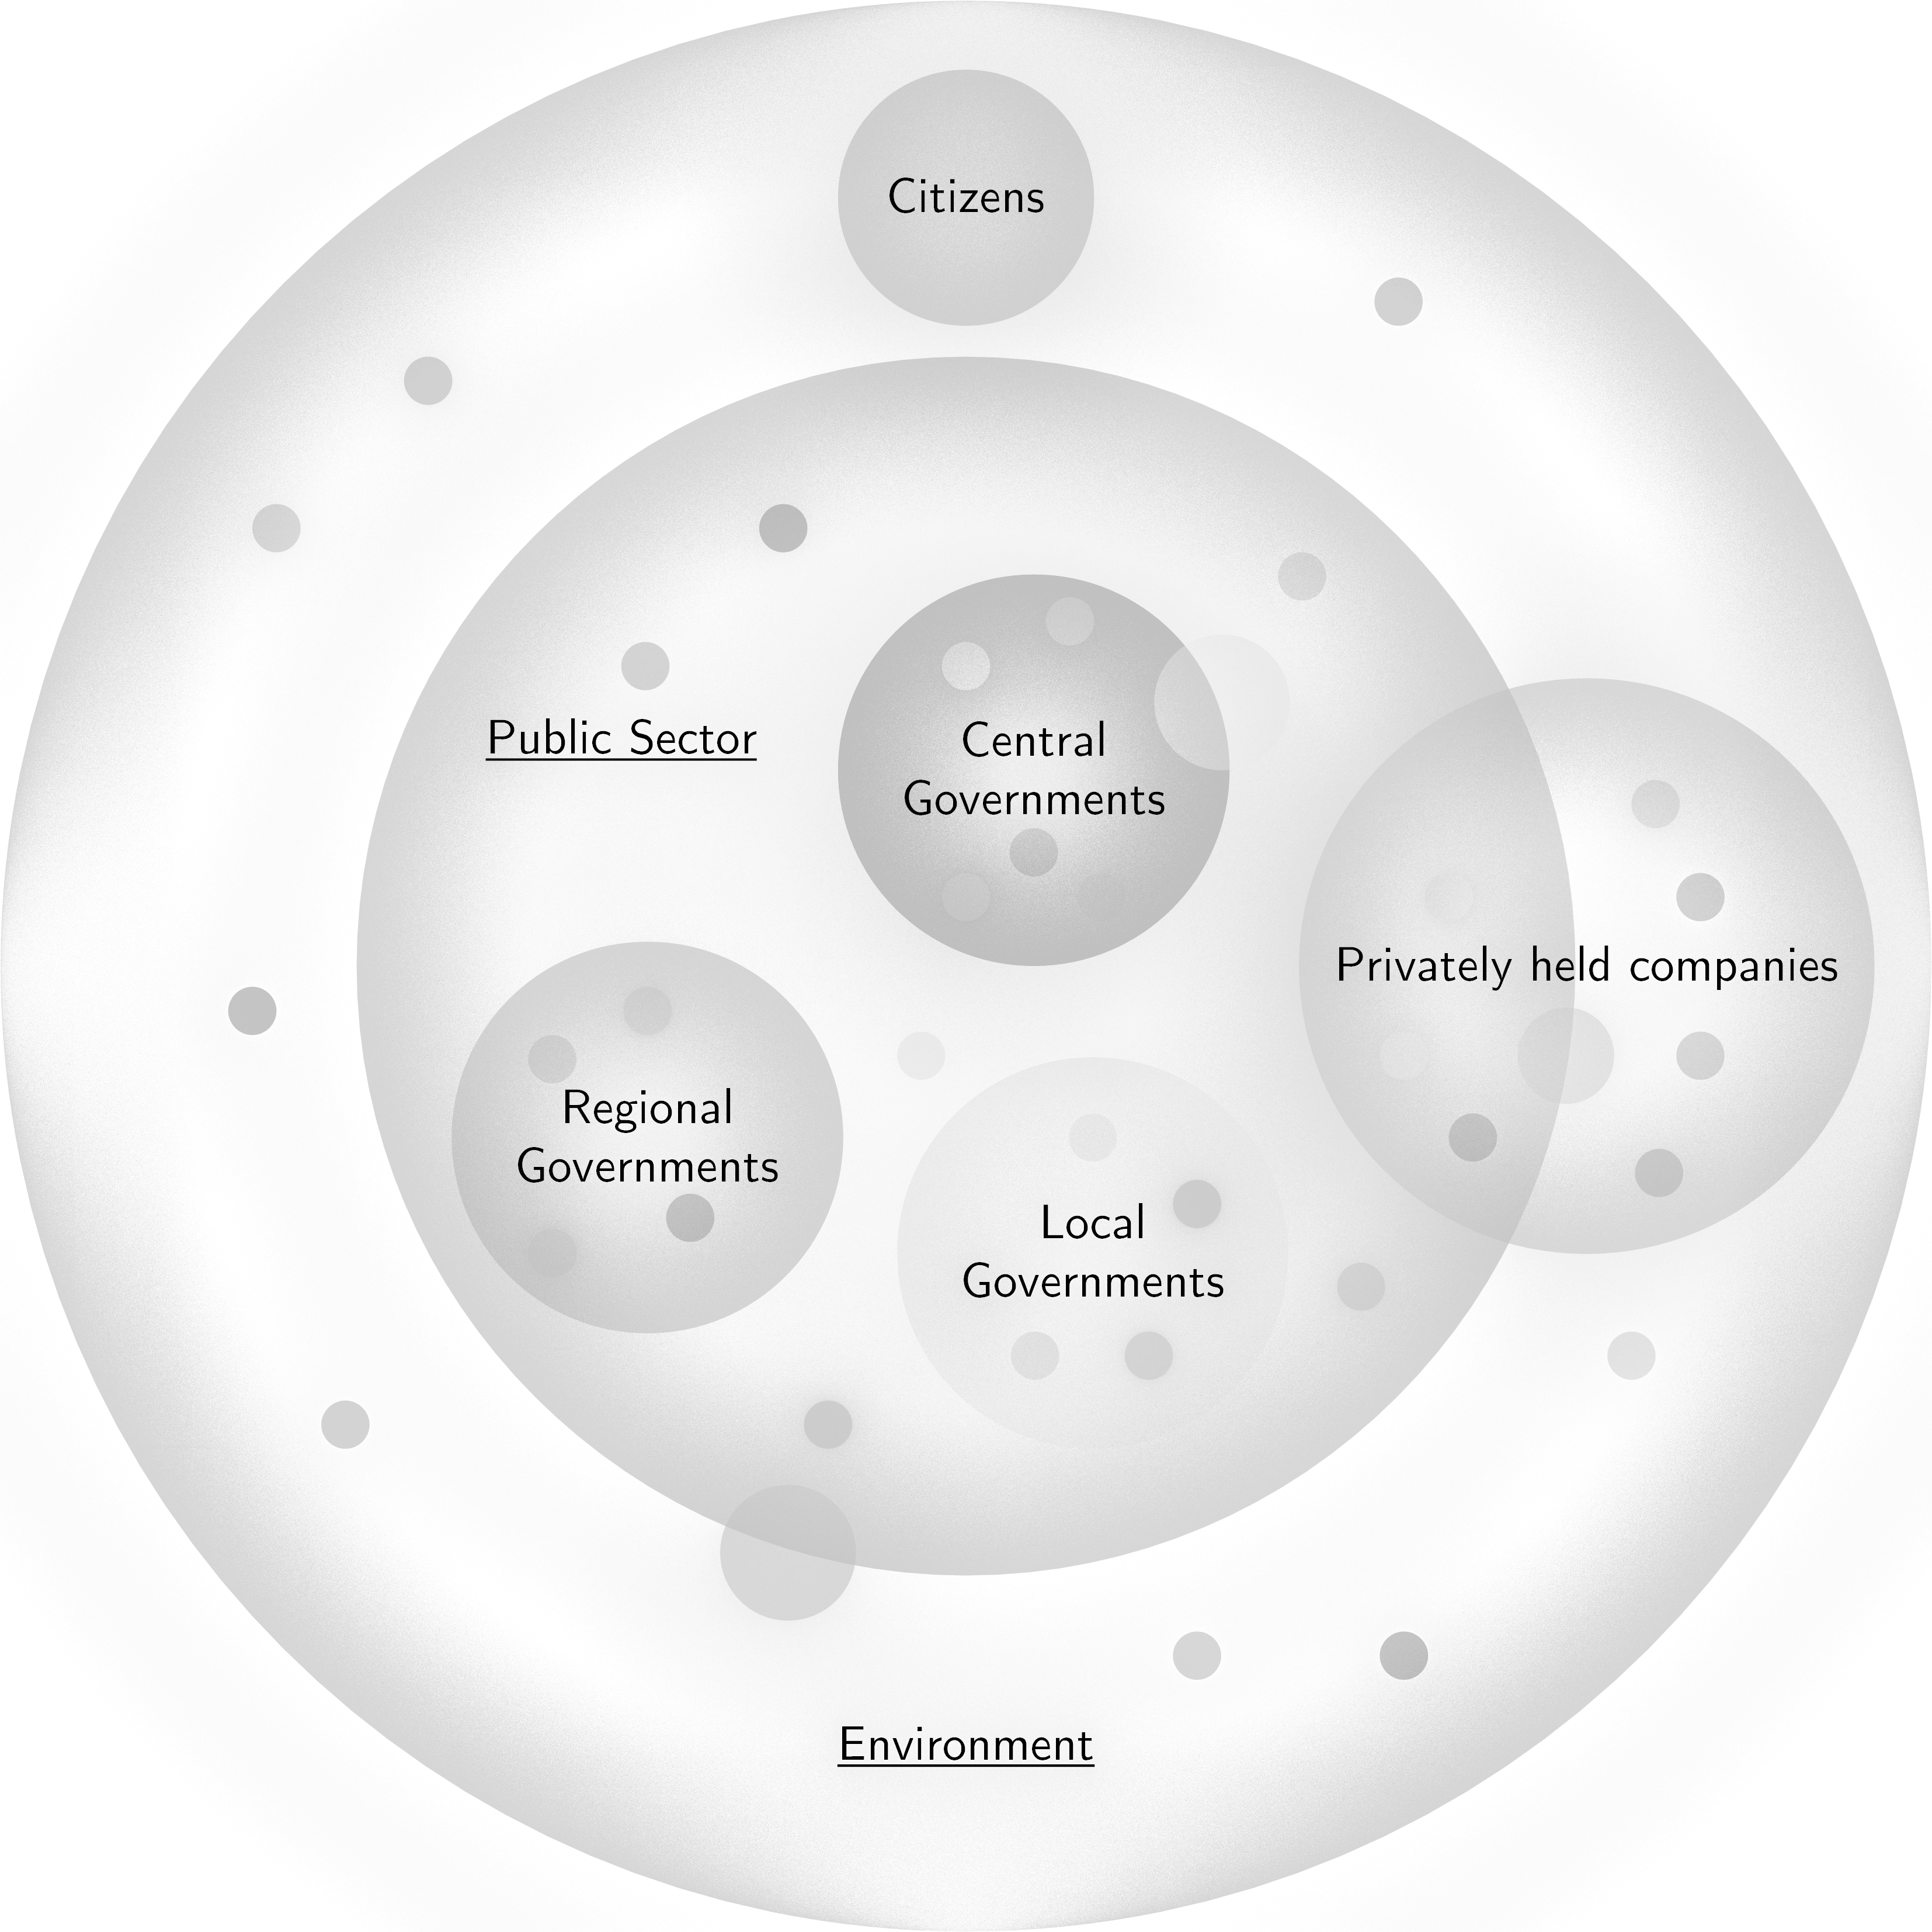
\includegraphics[width=0.5\linewidth]{images/pssystemofsystems}
	\caption[Public Sector as a \acrlong{sos}]{Public Sector as a \acrlong{sos}}
	\label{fig:pssystemofsystems}
\end{figure}

\section{Enterprise Architecture}
\label{sec:tbenterprisearchitecture}
This research is about which success factors positively influence \acrfull{ea} in achieving \gls{antifragility} in the \gls{ps}. This statement already assumes that \acrshort{ea} is a means to achieve a goal. Is this correct? Does the world have the same idea about \acrshort{ea}, or do they see it differently? Can \acrshort{ea} contribute to reaching the goals of an organisation or even a system? Regardless of the attention \acrshort{ea} gets, many researchers and practitioners have indicated that there is a lack of a shared mental model \parencite[p.~2]{SaintLouis2019}. The various definitions are not always complimentary, and sometimes they are even opposite \parencites{Hoogervorst2009}{Lapalme2012}{SaintLouis2019}.  A lens on Enterprise Architecture needs to be defined for this research to create a shared understanding of Enterprise Architecture. There is no shared mental model of Enterprise Architecture \parencite[p.~2]{SaintLouis2019}. The lack of a shared mental model can create confusion and conflicts concerning the purpose of Enterprise Architecture and its practice \parencite[p.~1]{SaintLouis2019}. The definitions vary in the scope of application. Some definitions only focus on IT systems, while others focus on the business, the enterprise, the environment, or any other combination. E.g. the definitions from \textcites{Gartner}{Graves2009}{Ross2014}{White2018}.
\vskip\baselineskip 
\begin{tcolorbox}[title=\textbf{Definition by \textcite{Gartner}}]
	\acrlong{ea} analyses the execution of change toward a desired business vision and outcomes. \acrlong{ea} leads the enterprise proactively and holistically, responding to disruptive forces.
\end{tcolorbox}
\vskip\baselineskip
\begin{tcolorbox}[title=\textbf{Definition by \textcite[p.~5]{Graves2009}}]
	\acrlong{ea} is the organising logic for business processes and IT infrastructure, reflecting its operating model's integration and standardisation requirements. It provides a long term view of a company's processes, systems and technologies so that individuals can build capabilities and not just fulfil immediate needs.
\end{tcolorbox}
\vskip\baselineskip
\begin{tcolorbox}[title=\textbf{Definition by \textcite[p.~9]{Ross2014}}]
	\acrlong{ea} is the organising logic for business processes and IT infrastructure, reflecting its operating model's integration and standardisation requirements. It provides a long term view of a company's processes, systems and technologies so that individuals can build capabilities and not just fulfil immediate needs.
\end{tcolorbox}
\vskip\baselineskip
\begin{tcolorbox}[title=\textbf{Definition by \textcite{White2018}}]
\acrlong{ea} is the process by which organizations standardize and organize IT infrastructure to aligns with business goals. These strategies support digital transformation, IT growth and the modernization of IT as a department. \acrshort{ea} is the practice of analysing, designing, planning and implementing enterprise analysis to successfully execute on business strategies. \acrshort{ea} helps to lay out how information, business and technology flow together.
\end{tcolorbox}
\vskip\baselineskip
All four Enterprise Architecture definition examples provide decision-support for direction and change at any level of the enterprise. E.g. ''The choices in the journey of an enterprise for an executive, the preferred technologies of process models for new developments for programme and portfolio management, as well planning when to decommission, change or replace systems'' \parencite[p.~4]{Graves2009}. Mature \acrshort{ea} can map interdependencies across almost every aspect of the enterprise \parencite[p.~5]{Graves2009}. A well defined and maintained \acrshort{ea} is proven to be a critical factor in an organisation's agility, effectiveness and ability to respond to risk, opportunity and change \parencite{Ross2014}. Enterprise Architecture assists in managing changes imposed on the organisation from the outside, by the market, by regulations, or at an operations level, by system failures, environmental incidents or customer complaints \parencite[p.~5]{Graves2009}. \acrshort{ea} can support re-designs and re-organisation, especially during significant organisational changes, mergers or acquisitions \parencite{White2018}. System development, IT Management, decision-making, and IT risk management are examples of capabilities supported by \acrshort{ea} \parencites{Graves2009}{Ross2014}{White2018}. Because a shared mental model is absent, there is also no clear approach to practising Enterprise Architecture \parencite[p.~2]{SaintLouis2019}.
\subsection{Approaches of Enterprise Architecture}
\label{sub:eaapproaches}
There are several perspectives to the practice of \acrshort{ea} \parencites{Lapalme2012}{Kotusev2015}{Ylinen2018}{Ylinen2020}. One of the perspectives is an approach that distinguishes two groups of \acrshort{ea} experts. A modelling-focused group forms a comprehensive view of an organisation, and a development-focused group using \acrshort{ea} for organisational development \parencites[p.~6]{Ylinen2020}. 
\begin{longtable}{p{.4\textwidth}p{.6\textwidth}}
	\toprule%
	\textbf{Approach} & \textbf{Description} \\%
	\midrule%
	\endhead%
	\hline
	\endfoot%
	\caption[Three approaches to Enterprise Architecture]{Three approaches to Enterprise Architecture}
	\label{tab:tbthreeapproaches}
	\endlastfoot%
	Traditional & A four-step sequential process. Document the current (as-is, baseline) state, develop the desired future (to-be, future) state and the transition plan to migrate from the current to the target state, and implement the plan and repeat the process. \\%
	\acrshort{mit} & Advocates the development of a long-term enterprise-level architectural vision to be translated into concrete project-level decisions through IT governance mechanisms. These decisions involve business and IT managers on different organisational levels. \\%
	\acrshort{dya} & ''Just enough, just in time'' architecture. The development of \acrshort{ea} starts no earlier than there is a need for it. Business initiatives trigger the activities of 
	\acrshort{ea} to make sure that needed projects fit nicely into the existing \acrshort{ea} and in the strategic plans of the enterprise. \\%
	\bottomrule%
\end{longtable}
However, another perspective distinguished three approaches \parencite[p.~4071]{Kotusev2015}. The traditional \parencite{Spewak1993}, the \acrfull{mit} \parencite{Ross2014}, and the \acrfull{dya} \parencite{Wagter2005} approach \parencite[p.~4071--4072]{Kotusev2015} (\cref{tab:tbthreeapproaches}). When you scrutinise the definitions of the three approaches, it becomes clear that the approaches are focused on organisations and not the environment. The \acrshort{ea} three schools of thought from \textcite{Lapalme2012} gives another perspective. Three possible schools of thought in the practice of \acrshort{ea} are, \gls{enterpriseitarchitecting}, \gls{enterpriseintegrating}, and \gls{enterpriseecologicaladaptation} \parencite[p.~38--41]{Lapalme2012} (\cref{tab:tbschoolsofthought,app:easchoolsproperties}).
\begin{longtable}{p{.4\textwidth}p{.6\textwidth}}
	\toprule%
	\textbf{Approach} & \textbf{Description} \\%
	\midrule%
	\endhead%
	\hline
	\endfoot%
	\caption[Enterprise Architecture schools of thought]{Enterprise Architecture schools of thought}
	\label{tab:tbschoolsofthought}
	\endlastfoot%
	\gls{enterpriseitarchitecting} & \acrshort{ea} is the glue between business and IT. \acrshort{ea} is an enabler for executing the business strategy. This school is about aligning an enterprise's IT assets to execute business strategy effectively and various operations using the proper IT capabilities. The school \gls{enterpriseitarchitecting} focuses on the IT capabilities while not questioning the business capabilities. \\%
	\gls{enterpriseintegrating} & \gls{enterpriseintegrating} links strategy and execution. It is not only enabling enterprise strategy it also implements it. Designing all the organisational dimensions is fostered with systems thinking. \gls{enterpriseintegrating} is aware of its environment and tries to manage the environment. \\%
	\gls{enterpriseecologicaladaptation} & \acrshort{ea} fosters organisational learning by designing all facets of the enterprise. It changes the environment and systematically designs the enterprise, including its relationship to the environment. The enterprise's relationship to its environment is an indisputably connected facet. This school of thought enables innovation and System-in-Environment adaptation. It looks for bidirectional incoherence between the enterprise and its environment. Nevertheless, it is the means for organisational innovation and sustainability. It is about enterprise and environment co-evolution. \\%
	\bottomrule%
\end{longtable}
\subsection{Defining Enterprise Architecture}
\label{sub:definingea}
\Gls{antifragile} deals with \glspl{stressor} and \glspl{blackswan} originating from the environment of the system of interest. The \acrlong{eaal} of \textcite{Botjes2021} fosters \gls{organisationallearning} and \gls{systemsthinking} capabilities to deal with \glspl{stressor} and \glspl{blackswan} \parencite[p.~2--4]{Botjes2021}. Exploring the \acrlong{ea} schools of thought \parencite{Lapalme2012} makes it clear that \textit{\gls{enterpriseecologicaladaptation}} is the best school in the context of \gls{antifragility}. \textit{\gls{enterpriseecologicaladaptation}} has a clear focus on the environment, fosters organisational and \gls{environmentallearning}, and embraces \gls{systemsthinking} \parencite[p.~40--41]{Lapalme2012}. Although the school \textit{\gls{enterpriseintegrating}} already has the notion of the environment, it is not changing the environment like the school \textit{\gls{enterpriseecologicaladaptation}}. At the same time, \textit{\gls{enterpriseitarchitecting}} has its main focus on the IT organisation of the enterprise itself. If an organisation want to survive in the turbulence of today's markets, the organisation must learn to adapt and innovate \parencite[p.~42]{Lapalme2012}. The school \textit{\gls{enterpriseecologicaladaptation}} is about adapt and innovate.

It is still necessary to define the definition of \acrshort{ea}. The lens of \acrshort{ea} is partly defined. \textit{'The how'} is known. The \acrlong{ea} school of thought \gls{enterpriseecologicaladaptation} is selected. The properties of this school are known (\cref{sec:propeea}). We still miss the definition of \acrshort{ea}. \textit{'The what'} is still unknown. \textcite[p~42]{Lapalme2012} mapped \acrlong{ea} authors to the three schools of thought (\cref{app:easchoolsresearchers}). These mappings were done based on the written literature.
\begin{table}[H]
	\centering
	\resizebox{\textwidth}{!}{%
	\begin{tabular}{p{0.4\textwidth}p{0.6\textwidth}}
		\toprule
		\textbf{Author(s)} & \textbf{Description} \\%
		\midrule
		Jamshid Gharajedaghi & \textcite{Gharajedaghi2011} \\%
		Tom Graves & \textcite{Graves2008} \\%
		Jan Hoogervorst	& \textcite{Hoogervorst2009} \\%
		James Martin & \textcite{Martin1995} \\%
		Kevin Smith and Tom Graves & \textcite{Smith2011} \\%
		James Lapalme and Donald de Guerre & \textcite{Lapalme2012b} \\%
		\bottomrule
	\end{tabular}
	}%
	\caption[Authors of Enterprise Ecological Adaptation]{Authors of Enterprise Ecological Adaptation}
	\label{tab:eeaauthors}
\end{table}
Following the Enterprise Architecture school of thought of Enterprise Ecological Adaptation, the most likely author for a definition of Enterprise Architecture is \textcite{Graves2008} (\cref{tab:eeaauthors}). The most basic definition of Enterprise Architecture is that ''Enterprise Architecture is the integration of everything the enterprise is and does'' \parencite[p.~1]{Graves2008}. Enterprise Architecture is about the architecture (the structure) of the whole of the enterprise. Instead, the whole than a single sub-system. There are no simple states of 'as is' and 'to be'. The world is dynamic and not static. Everything in a business system depends on everything else \parencite[p.~14]{Graves2008}. 


With level 4 as the highest maturity level 

integration across entire enterprise: increase adaptability, resilience, management of opportunity / risk; increase synergies between processes and partners \parencites[p.9--10]{Bredemeyer2003}[p.~4--5]{Malan2005}[p.~14--15]{Graves2008}. Again this has references to the environment.